\documentclass{beamer}\usepackage[]{graphicx}\usepackage[]{xcolor}
% maxwidth is the original width if it is less than linewidth
% otherwise use linewidth (to make sure the graphics do not exceed the margin)
\makeatletter
\def\maxwidth{ %
  \ifdim\Gin@nat@width>\linewidth
    \linewidth
  \else
    \Gin@nat@width
  \fi
}
\makeatother

\definecolor{fgcolor}{rgb}{0.345, 0.345, 0.345}
\newcommand{\hlnum}[1]{\textcolor[rgb]{0.686,0.059,0.569}{#1}}%
\newcommand{\hlstr}[1]{\textcolor[rgb]{0.192,0.494,0.8}{#1}}%
\newcommand{\hlcom}[1]{\textcolor[rgb]{0.678,0.584,0.686}{\textit{#1}}}%
\newcommand{\hlopt}[1]{\textcolor[rgb]{0,0,0}{#1}}%
\newcommand{\hlstd}[1]{\textcolor[rgb]{0.345,0.345,0.345}{#1}}%
\newcommand{\hlkwa}[1]{\textcolor[rgb]{0.161,0.373,0.58}{\textbf{#1}}}%
\newcommand{\hlkwb}[1]{\textcolor[rgb]{0.69,0.353,0.396}{#1}}%
\newcommand{\hlkwc}[1]{\textcolor[rgb]{0.333,0.667,0.333}{#1}}%
\newcommand{\hlkwd}[1]{\textcolor[rgb]{0.737,0.353,0.396}{\textbf{#1}}}%
\let\hlipl\hlkwb

\usepackage{framed}
\makeatletter
\newenvironment{kframe}{%
 \def\at@end@of@kframe{}%
 \ifinner\ifhmode%
  \def\at@end@of@kframe{\end{minipage}}%
  \begin{minipage}{\columnwidth}%
 \fi\fi%
 \def\FrameCommand##1{\hskip\@totalleftmargin \hskip-\fboxsep
 \colorbox{shadecolor}{##1}\hskip-\fboxsep
     % There is no \\@totalrightmargin, so:
     \hskip-\linewidth \hskip-\@totalleftmargin \hskip\columnwidth}%
 \MakeFramed {\advance\hsize-\width
   \@totalleftmargin\z@ \linewidth\hsize
   \@setminipage}}%
 {\par\unskip\endMakeFramed%
 \at@end@of@kframe}
\makeatother

\definecolor{shadecolor}{rgb}{.97, .97, .97}
\definecolor{messagecolor}{rgb}{0, 0, 0}
\definecolor{warningcolor}{rgb}{1, 0, 1}
\definecolor{errorcolor}{rgb}{1, 0, 0}
\newenvironment{knitrout}{}{} % an empty environment to be redefined in TeX

\usepackage{alltt}
\usepackage{graphicx}
% \usepackage{comment}

\usepackage{graphicx}
\usepackage{verbatim}
\usepackage{etoolbox}
\usepackage{everysel}
% \usepackage{enumitem}

%% This package allows text highlighting
\usepackage{soul}

%% This sets the theme of the presentation which controls
%% the formatting of the slides
\usetheme{Boadilla}

%% Turn off the navigation symbols
\setbeamertemplate{navigation symbols}{} 

%% Change the default itemize [ball]s to [circle]s
\setbeamertemplate{itemize items}[circle]

%% Change the default enumerate [ball]s to plain text
\setbeamertemplate{enumerate items}[default]

%% Load the enumitem package and ensure it works nicely with beamer
% \setitemize{label=\usebeamerfont*{itemize item}
%   \usebeamercolor[fg]{itemize item}
%   \usebeamertemplate{itemize item}}
% \setenumerate{label=\usebeamerfont*{enumerate item}
%   \usebeamercolor[fg]{enumerate item}
%   \usebeamertemplate{enumerate item}}

%% Set the author block so STATS 201/8 appears on every
\author{STATS 201/8}

%% Clear the date block
\date{}


\setbeamercolor{title}{bg=blue!40}
\setbeamerfont{title}{size=\LARGE,series=\bfseries}

%%Sectioning commands
\setbeamercolor{section title}{bg=blue!20}
\setbeamerfont{section title}{size=\large}

\setbeamertemplate{section page}{%
    \begingroup
        \begin{beamercolorbox}[sep=10pt,center,rounded=true,shadow=true]{section title}
        \usebeamerfont{section title}Section~\thechapter.\thesection \newline \insertsection\par
        \end{beamercolorbox}
		\vfill
    \endgroup
}

\newcommand{\BeginSection}[1]{\section{#1} \frame{\sectionpage}}
%\AtBeginSection[]{%
%    \begin{frame}
%        \sectionpage
%    \end{frame}
%}


%% This makes all equations blue
\AtBeginEnvironment{equation*}{\color{blue}}
\AtBeginEnvironment{align*}{\color{blue}}
\everymath{\color{blue}}

%% This puts a 0 point space between paragraphs, means we don't need to use vspace, or list environments if 
%% we don't want to
\setlength{\parskip}{0pt}


%% Russell: removes spaces after R input/output?
\setlength{\topsep}{0.5mm}

%% David: In addition to Russel's command to remove spaces after R input/output, these commands remove the space between R input/output.
%% Stackoverflow link: https://stackoverflow.com/questions/35734525/reduce-space-between-code-chunks-and-code-output-in-rmarkdown-beamer-presentatio
%% \setlength{\OuterFrameSep}{-2pt}
\makeatletter
\preto{\@verbatim}{\topsep=-1pt \partopsep=-1pt }
\makeatother

%% Some useful colors
\definecolor{darkgreen}{rgb}{0.176,0.486,0.031}
\definecolor{redbrown}{HTML}{950605}
\definecolor{darkred}{HTML}{d80605}


%% nice little macro for changing the font of R code
\newcommand{\rcode}[1]{\protect{\color{darkgreen}\texttt{#1}}}

%% macro for bold blue italics
\newcommand{\blueBoldEmph}[1]{{\color{blue}\textbf{\emph{#1}}}}

% ~iid macro
\newcommand{\iid }{\stackrel{iid}{\sim}}

%% Macro for t-test amd P-value
\newcommand{\ttest}{\emph{t}-test}
\newcommand{\pval}{\emph{P}-value}

%% Statistics operators 
\DeclareMathOperator{\Bias}{Bias}
\DeclareMathOperator{\Cov}{Cov}
\DeclareMathOperator*{\Cor}{Cor}
\DeclareMathOperator{\E}{E}
\DeclareMathOperator{\MSE}{MSE}
\DeclareMathOperator{\Odds}{Odds}
\DeclareMathOperator{\OR}{OR}
\DeclareMathOperator{\PMSE}{PMSE}
\DeclareMathOperator{\sd}{sd}
\DeclareMathOperator{\se}{se}
\DeclareMathOperator*{\Var}{Var}
\DeclareMathOperator{\logit}{logit}

%% Should see if can make this a mathop
\newcommand{\comb}[2]{\mbox{$\big(_{#2}^{#1}\big)$}}






\IfFileExists{upquote.sty}{\usepackage{upquote}}{}
\begin{document}
\newcommand{\thechapter}{8}

\title{Chapter 8: \\ Linear models with both numeric and factor explanatory variables \\~\\ Part 1: The interaction model}
\institute{University of Auckland}


\begin{frame}
\titlepage
\end{frame}


\begin{frame}[t]
\frametitle{Learning Outcomes}
In this chapter you will learn about:
\begin{center}
\vspace{16pt}
  \begin{itemize}
  \item Models which contain categorical and numeric explanatory variables\footnote{Models of this type are commonly known as Analysis of Covariance models, which is abbreviated to ANCOVA. }
    \item Useful plots to display the data
    \item The meaning of {\bf interaction}
    \item Fitting a model with an interaction term
    \item Interpretting the fitted model
    \item Relevant \rcode{R}-code.
  \end{itemize}
\end{center}

\end{frame}


%%%%%%%%%%%%%%%%%%%%%%%%%%%%%%%%%%%%%%%%%%%%%%%%%%%%%%%%%%%%%%%%%%%%%%%%%%%%%%%%%%%%%%%%%%%
\BeginSection{Example: Using both test score and attendance to explain exam score  \\~\\ Part A: Exploratory analysis}
%%%%%%%%%%%%%%%%%%%%%%%%%%%%%%%%%%%%%%%%%%%%%%%%%%%%%%%%%%%%%%%%%%%%%%%%%%%%%%%%%%%%%%%%%%%


\begin{frame}[fragile]
\frametitle{Example -- Exam vs.\ test \textbf{and} attendance}
We have have learnt how to deal with the effect of test mark on exam score,
and of attendance on exam score, individually.\\
\bigskip
So what is stopping us from using both? Absolutely nothing. \\
\bigskip
Let's begin by visualizing how test score relates to the exam score for the attenders and the non-attenders.

\begin{knitrout}\scriptsize
\definecolor{shadecolor}{rgb}{0.969, 0.969, 0.969}\color{fgcolor}\begin{kframe}
\begin{alltt}
\hlstd{> }\hlcom{## Invoke the s20x library}
\hlstd{> }\hlcom{#library(s20x)}
\hlstd{> }\hlcom{## Importing data into R}
\hlstd{> }\hlstd{Stats20x.df} \hlkwb{=} \hlkwd{read.table}\hlstd{(}\hlstr{"Data/STATS20x.txt"}\hlstd{,} \hlkwc{header}\hlstd{=T)}
\hlstd{> }\hlstd{Stats20x.df}\hlopt{$}\hlstd{Attend}\hlkwb{=}\hlkwd{as.factor}\hlstd{(Stats20x.df}\hlopt{$}\hlstd{Attend)}
\hlstd{> }\hlcom{## Plot blue "Y" for "Yes" (regular attenders), and red "N" for "No"}
\hlstd{> }\hlkwd{plot}\hlstd{(Exam} \hlopt{~} \hlstd{Test,}\hlkwc{data} \hlstd{= Stats20x.df,}\hlkwc{pch}\hlstd{=}\hlkwd{substr}\hlstd{(Attend,}\hlnum{1}\hlstd{,}\hlnum{1}\hlstd{),}
\hlstd{+ }        \hlkwc{col}\hlstd{=}\hlkwd{ifelse}\hlstd{(Attend}\hlopt{==}\hlstr{"Yes"}\hlstd{,}\hlstr{"blue"}\hlstd{,}\hlstr{"red"}\hlstd{))}
\end{alltt}
\end{kframe}
\end{knitrout}
%plot(Exam ~ Test,data = Stats20x.df,pch=substr(Attend,1,1))

\end{frame}

\begin{frame}[fragile]
\frametitle{Exam vs.\ test \textbf{and} attendance\ldots}



\begin{figure}
  \centering
  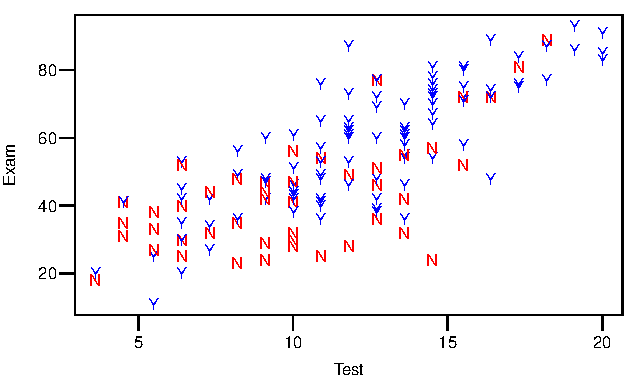
\includegraphics{figure/RC-H08-002}
\end{figure}

The above plot is a bit cluttered, so we could also draw a plot for each attendance type. For the sake of comparison it is important to ensure that the horizontal and vertical limits of the two scatter plots are the same.

\end{frame}


\begin{frame}[fragile]
\frametitle{Exam vs.\ test \textbf{and} attendance\ldots}

Here is the plot for the regular attenders.

\begin{knitrout}\scriptsize
\definecolor{shadecolor}{rgb}{0.969, 0.969, 0.969}\color{fgcolor}\begin{kframe}
\begin{alltt}
\hlstd{> }\hlstd{Attendees.df} \hlkwb{=} \hlkwd{subset}\hlstd{(Stats20x.df, Attend} \hlopt{==} \hlstr{"Yes"}\hlstd{)}
\hlstd{> }\hlkwd{plot}\hlstd{(Exam} \hlopt{~} \hlstd{Test,} \hlkwc{data} \hlstd{= Attendees.df,} \hlkwc{xlim} \hlstd{=} \hlkwd{c}\hlstd{(}\hlnum{0}\hlstd{,} \hlnum{20}\hlstd{),} \hlkwc{ylim} \hlstd{=} \hlkwd{c}\hlstd{(}\hlnum{0}\hlstd{,} \hlnum{100}\hlstd{),}
\hlstd{+ }     \hlkwc{pch} \hlstd{=} \hlstr{"Y"}\hlstd{,} \hlkwc{cex} \hlstd{=} \hlnum{0.7}\hlstd{)}
\end{alltt}
\end{kframe}
\end{knitrout}



\begin{figure}
  \centering
  \includegraphics{figure/RC-H08-004}
\end{figure}

\end{frame}


\begin{frame}[fragile]
\frametitle{Exam vs.\ test \textbf{and} attendance\ldots}
Here is the plot for the non-attenders.

\begin{knitrout}\scriptsize
\definecolor{shadecolor}{rgb}{0.969, 0.969, 0.969}\color{fgcolor}\begin{kframe}
\begin{alltt}
\hlstd{> }\hlstd{Absentees.df} \hlkwb{=} \hlkwd{subset}\hlstd{(Stats20x.df, Attend} \hlopt{==} \hlstr{"No"}\hlstd{)}
\hlstd{> }\hlkwd{plot}\hlstd{(Exam} \hlopt{~} \hlstd{Test,} \hlkwc{data} \hlstd{= Absentees.df,} \hlkwc{xlim} \hlstd{=} \hlkwd{c}\hlstd{(}\hlnum{0}\hlstd{,} \hlnum{20}\hlstd{),} \hlkwc{ylim} \hlstd{=} \hlkwd{c}\hlstd{(}\hlnum{0}\hlstd{,} \hlnum{100}\hlstd{),}
\hlstd{+ }     \hlkwc{pch} \hlstd{=} \hlstr{"N"}\hlstd{,} \hlkwc{cex} \hlstd{=} \hlnum{0.7}\hlstd{)}
\end{alltt}
\end{kframe}
\end{knitrout}




\begin{figure}
  \centering
  \includegraphics{figure/RC-H08-006}
\end{figure}

\end{frame}



\begin{frame}[fragile]
\frametitle{Exam vs.\ test \textbf{and} attendance\ldots}
Also, there seems to be some non-attenders who do well in the test and exam so we could (and will) see whether we should include these people. 
They are identified in red (stars) with the \rcode{R} code below.

\begin{knitrout}\scriptsize
\definecolor{shadecolor}{rgb}{0.969, 0.969, 0.969}\color{fgcolor}\begin{kframe}
\begin{alltt}
\hlstd{> }\hlkwd{plot}\hlstd{(Exam} \hlopt{~} \hlstd{Test,} \hlkwc{data} \hlstd{= Absentees.df,} \hlkwc{xlim} \hlstd{=} \hlkwd{c}\hlstd{(}\hlnum{0}\hlstd{,} \hlnum{20}\hlstd{),} \hlkwc{ylim} \hlstd{=} \hlkwd{c}\hlstd{(}\hlnum{0}\hlstd{,} \hlnum{100}\hlstd{),}
\hlstd{+ }     \hlkwc{cex} \hlstd{=} \hlnum{0.7}\hlstd{,} \hlkwc{col} \hlstd{=} \hlkwd{ifelse}\hlstd{(Absentees.df}\hlopt{$}\hlstd{Test} \hlopt{<=}\hlnum{16} \hlstd{,} \hlstr{"black"}\hlstd{,} \hlstr{"red"}\hlstd{),}
\hlstd{+ }     \hlkwc{pch} \hlstd{=} \hlkwd{ifelse}\hlstd{(Absentees.df}\hlopt{$}\hlstd{Test} \hlopt{<=}\hlnum{16} \hlstd{,} \hlnum{1}\hlstd{,} \hlnum{8}\hlstd{))}
\end{alltt}
\end{kframe}
\end{knitrout}


\begin{figure}
  \centering
  \includegraphics{figure/RC-H08-008}
\end{figure}

% Whether or not we include them, we will discuss later.

\end{frame}


\begin{frame}[fragile]
\frametitle{Exam vs.\ test \textbf{and} attendance\ldots}
Hmmm---it seems that the non-attenders may get less `return on investment' on test efforts compared to the regular attenders. \\
\bigskip
What we mean is that is that the slope looks less steep for non-attenders than regular attenders.\\
\bigskip 
Can we explore this idea with a linear model? \textbf{Yes!}
\end{frame}



%%%%%%%%%%%%%%%%%%%%%%%%%%%%%%%%%%%%%%%%%%%%%%%%%%%%%%%%%%%%%%%%%%%%%%%%%%%%%%%%%%%%%%%%%%%
\BeginSection{Example: Using both test score and attendance to explain exam score  \\~\\ Part B: Fitting the linear model}
%%%%%%%%%%%%%%%%%%%%%%%%%%%%%%%%%%%%%%%%%%%%%%%%%%%%%%%%%%%%%%%%%%%%%%%%%%%%%%%%%%%%%%%%%%%


\begin{frame}[fragile]
\frametitle{Exam vs.\ test \textbf{and} attendance\ldots}
So, it looks like we need to fit two different lines depending on whether the student is a regular attender or not.\\
\bigskip
One approach would be to fit separate linear models to the data in the
\rcode{Attendees.df} and \rcode{Absentees.df} dataframes. 
However, this approach limits the questions that we can answer.\\
\bigskip
A more powerful approach is to use a single \rcode{lm} model to fit the two lines.\\
\bigskip
We can do this by using indicator variables (recall Chap 5). \\
\bigskip
Let us recode attendance using an indicator variable to indicate whether the student was an attender or not. 
\end{frame}


\begin{frame}[fragile]
\frametitle{Exam vs.\ test \textbf{and} attendance\ldots}
We will call our indicator variable \rcode{D} for greater convenience of notation.\footnote{Last time (see Chapter 5) we called this indicator variable \rcode {Attend2} -- but \rcode{D} is easier to use in an equation.}\\
\bigskip
\begin{knitrout}\scriptsize
\definecolor{shadecolor}{rgb}{0.969, 0.969, 0.969}\color{fgcolor}\begin{kframe}
\begin{alltt}
\hlstd{> }\hlcom{## Boolean statement if Attend ="Yes" (TRUE) D=1, othwerwise 0 (FALSE);}
\hlstd{> }\hlstd{Stats20x.df}\hlopt{$}\hlstd{D} \hlkwb{=} \hlkwd{as.numeric}\hlstd{(Stats20x.df}\hlopt{$}\hlstd{Attend}\hlopt{==}\hlstr{"Yes"}\hlstd{)}
\hlstd{> }\hlkwd{table}\hlstd{(Stats20x.df}\hlopt{$}\hlstd{Attend, Stats20x.df}\hlopt{$}\hlstd{D)} \hlcom{## Check it is okay}
\end{alltt}
\begin{verbatim}
     
        0   1
  No   46   0
  Yes   0 100
\end{verbatim}
\end{kframe}
\end{knitrout}
% \bigskip
% \textbf{R Note:} The coursebook uses \rcode{within} to achieve the same result. There are various schools of thought in the R community about whether we should use \rcode{within}. We can achieve the same result by making an assignment to a new variable (as we have done above) and the code is simpler. Therefore we will not use \rcode{within} in this course, but we will not stop you from using it if you want to. 
\end{frame}


\begin{frame}[fragile]
\frametitle{Exam vs.\ test \textbf{and} attendance\ldots}
\framesubtitle{Formulating the model}
Our straight line model for the non-attenders (i.e., \rcode{D = 0}) students will be:\\
\bigskip
\[
Exam=\beta_0 + \beta_1\times \rcode{Test} + \varepsilon \mbox{ where } \varepsilon \iid N(0, \sigma^2).
\]
\bigskip

We would expect some benefit from doing better in the test, 
so we would suspect that $\beta_1>0$. The null hypothesis is, as usual, 
\[
H_0:\beta_1=0.
\]
\end{frame}


\begin{frame}[fragile]
\frametitle{Exam vs.\ test \textbf{and} attendance\ldots}
\framesubtitle{Formulating the model\ldots}
From the scatter plots we suspect there may be a different slope value for the regular attenders (in fact steeper, i.e., greater positive value.) \\
\bigskip
So what we are saying is that the slope for attenders is the slope for non-attenders plus a positive number so that it increases the slope.\\
\bigskip
We will call this additional (positive) number $\beta_3$.\footnote{ The choice of symbol $\beta_3$ will be come obvious soon.}\\
\bigskip
So we can say that the slope for any student is:
\[
\beta_1+D\times\beta_3
\]
where \rcode{D = 0} when the student is a non-attender and  \rcode{D = 1} when they attend regularly.
\end{frame}


\begin{frame}[fragile]
\frametitle{Exam vs.\ test \textbf{and} attendance\ldots}
\framesubtitle{Formulating the model\ldots}
For the non-attenders (\rcode{D = 0}) the slope is:
\begin{align*}
\beta_1 + D \times \beta_3 &=\beta_1+ 0 \times \beta_3\\
&=\beta_1.
\end{align*}
For the regular attenders (\rcode{D = 1}) the slope is:
\begin{align*}
\beta_1+1\times\beta_3&=\beta_1+1\times\beta_3\\
&=\beta_1+\beta_3.
\end{align*}
We suspect that $\beta_3>0$.
The null hypothesis, as usual, is $H_0: \beta_3=0$.

The scatter plots suggest that the slope associated with \rcode{Test} changes depending on whether the student attends or not. This idea is known as interaction. That is, the effect of \rcode{Test} interacts with the students' attendance behaviour. 

\medskip
In our example, students who attend regularly, we suspect, get `more' from the \rcode{Test} than  non-attenders.
\end{frame}


\begin{frame}[fragile]
\frametitle{Exam vs.\ test \textbf{and} attendance\ldots}
\framesubtitle{Formulating the model\ldots}
The intercept for both groups can be formulated in a similar way. That is: 
\[
\beta_0+D \times \beta_2.
\]
\medskip
So, for the non-attenders (\rcode{D = 0}) the intercept is $\beta_0$. 

\medskip
For the regular attenders (\rcode{D = 1}): the intercept is $\beta_0+\beta_2$.

\bigskip
We do not have much interest in the intercept terms if the equal slope hypothesis ($H_0: \beta_3=0$) is rejected\footnote{If the equal slope hypothesis is {\bf not} rejected then we {\bf do} have interest in $\beta_2$ since it is then the difference between attenders and non-attenders for any given test score}, since they give the expected exam scores for students who get zero test score. So, we would then not be interested in testing $H_0: \beta_2=0$.

\end{frame}


\begin{frame}[fragile]
\frametitle{Exam vs.\ test \textbf{and} attendance\ldots}
\framesubtitle{Formulating the model\ldots}
So, our model is:
\begin{align*}
\rcode{Exam} 
 &= \beta_0 + \beta_2 \times D + ( \beta_1 + \beta_3 \times D) \rcode{Test} + \varepsilon \\
 &= (\beta_0 + \beta_2 \times D) + (\beta_1 + \beta_3\times D)\rcode{Test} + \varepsilon\\
 &= \beta_0 + \beta_1\times \rcode{Test} + \beta_2 \times D + \beta_3\times D\times \rcode{Test} + \varepsilon\\
\end{align*}
In order to fit this model we create an additional explanatory variable $D \times \rcode{Test}$.\\
\bigskip
\begin{knitrout}\scriptsize
\definecolor{shadecolor}{rgb}{0.969, 0.969, 0.969}\color{fgcolor}\begin{kframe}
\begin{alltt}
\hlstd{> }\hlstd{Stats20x.df}\hlopt{$}\hlstd{TestD}  \hlkwb{=} \hlkwd{with}\hlstd{(Stats20x.df, \{TestD} \hlkwb{=} \hlstd{D} \hlopt{*} \hlstd{Test\})}
\hlstd{> }\hlstd{TestAttend.fit} \hlkwb{=} \hlkwd{lm}\hlstd{(Exam} \hlopt{~} \hlstd{Test} \hlopt{+} \hlstd{D} \hlopt{+} \hlstd{TestD,} \hlkwc{data} \hlstd{= Stats20x.df)}
\end{alltt}
\end{kframe}
\end{knitrout}
\end{frame}



\begin{frame}[fragile]
\frametitle{Exam vs.\ test \textbf{and} attendance\ldots}
\framesubtitle{Assumption checks}

\begin{knitrout}\scriptsize
\definecolor{shadecolor}{rgb}{0.969, 0.969, 0.969}\color{fgcolor}\begin{kframe}
\begin{alltt}
\hlstd{> }\hlkwd{plot}\hlstd{(TestAttend.fit,}\hlkwc{which}\hlstd{=}\hlnum{1}\hlstd{)}
\end{alltt}
\end{kframe}
\end{knitrout}



\begin{figure}
  \centering
  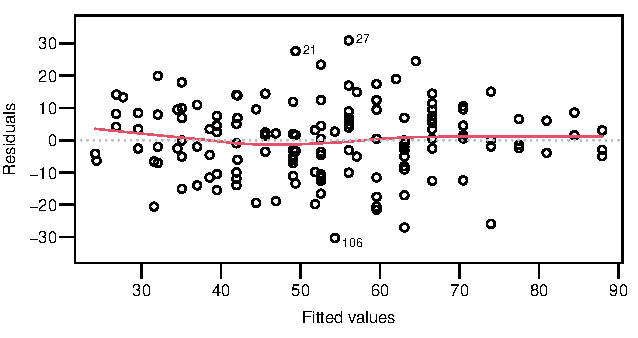
\includegraphics{figure/RC-H08-012}
\end{figure}

This looks okay. There is a narrowing at the higher values of fit, but there are fewer observations there.
\end{frame}




\begin{frame}[fragile]
\frametitle{Exam vs.\ test \textbf{and} attendance\ldots}
\framesubtitle{Assumption checks\ldots}

\begin{knitrout}\scriptsize
\definecolor{shadecolor}{rgb}{0.969, 0.969, 0.969}\color{fgcolor}\begin{kframe}
\begin{alltt}
\hlstd{> }\hlkwd{normcheck}\hlstd{(TestAttend.fit)}
\end{alltt}
\end{kframe}
\end{knitrout}



\begin{figure}
  \centering
  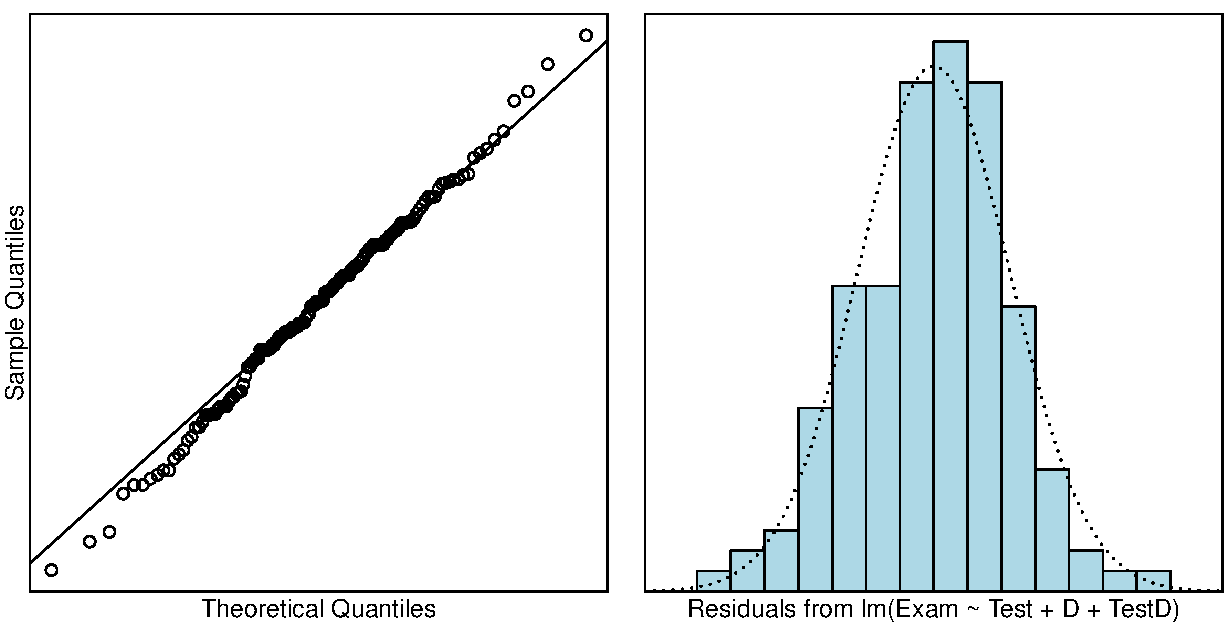
\includegraphics[scale=0.5]{figure/RC-H08-014}
\end{figure}

The normality assumption seems fine.
\end{frame}


\begin{frame}[fragile]
\frametitle{Exam vs.\ test \textbf{and} attendance\ldots}
\framesubtitle{Assumption checks\ldots}

\begin{knitrout}\scriptsize
\definecolor{shadecolor}{rgb}{0.969, 0.969, 0.969}\color{fgcolor}\begin{kframe}
\begin{alltt}
\hlstd{> }\hlkwd{cooks20x}\hlstd{(TestAttend.fit)}
\end{alltt}
\end{kframe}
\end{knitrout}



\begin{figure}
  \centering
  \includegraphics[scale=0.5]{figure/RC-H08-016}
\end{figure}

No unduly influential points here.
\end{frame}



\begin{frame}[fragile]
\frametitle{Exam vs.\ test \textbf{and} attendance\ldots}
\framesubtitle{Let us look at the fit}

\medskip
We can now trust the fitted \rcode{lm}.
The summary output is:

\begin{knitrout}\scriptsize
\definecolor{shadecolor}{rgb}{0.969, 0.969, 0.969}\color{fgcolor}\begin{kframe}
\begin{alltt}
\hlstd{> }\hlkwd{summary}\hlstd{(TestAttend.fit)}
\end{alltt}
\end{kframe}
\end{knitrout}

\begin{knitrout}\scriptsize
\definecolor{shadecolor}{rgb}{0.969, 0.969, 0.969}\color{fgcolor}\begin{kframe}
\begin{verbatim}
Coefficients:
            Estimate Std. Error t value Pr(>|t|)    
(Intercept)  14.4467     4.9443   2.922  0.00405 ** 
Test          2.7496     0.4603   5.973 1.78e-08 ***
D            -4.2582     6.3723  -0.668  0.50506    
TestD         1.1380     0.5577   2.040  0.04316 *  
---
Residual standard error: 11.41 on 142 degrees of freedom
Multiple R-squared:  0.6347,	Adjusted R-squared:  0.627 
F-statistic: 82.25 on 3 and 142 DF,  p-value: < 2.2e-16
\end{verbatim}
\end{kframe}
\end{knitrout}

\textbf{Note} that the coefficient for \rcode{TestD} is significant which means our 
intuition seem correct. That is, the regular attenders do get a `greater return' on their \rcode{Test} `investment'.
\end{frame}


\begin{frame}[fragile]
\frametitle{Exam vs.\ test \textbf{and} attendance\ldots}
\framesubtitle{Making sense of it all}
Let's take a closer look at the model we have just fitted. We will produce a separate plot for each attender group.\\
\bigskip
\textbf{Recall:} \rcode{D = 0} if the student was a non-attender (the baseline level).\\
\bigskip
Therefore, the estimated coefficients that are associated with non-attenders are $\hat{\beta}_0$ and $\hat{\beta}_1$:\\
\bigskip
\begin{knitrout}\scriptsize
\definecolor{shadecolor}{rgb}{0.969, 0.969, 0.969}\color{fgcolor}\begin{kframe}
\begin{alltt}
\hlstd{> }\hlkwd{coef}\hlstd{(TestAttend.fit)[}\hlnum{1}\hlopt{:}\hlnum{2}\hlstd{]}
\end{alltt}
\begin{verbatim}
(Intercept)        Test 
  14.446750    2.749568 
\end{verbatim}
\end{kframe}
\end{knitrout}
\end{frame}


\begin{frame}[fragile]
\frametitle{Exam vs.\ test \textbf{and} attendance\ldots}
\framesubtitle{Making sense of it all\ldots}
Here is the \rcode{R} code for a plot of the non-attender group with their fitted line (\rcode{D = 0}).
\begin{knitrout}\scriptsize
\definecolor{shadecolor}{rgb}{0.969, 0.969, 0.969}\color{fgcolor}\begin{kframe}
\begin{alltt}
\hlstd{> }\hlkwd{plot}\hlstd{(Exam}\hlopt{~}\hlstd{Test,}\hlkwc{data}\hlstd{=Absentees.df,}\hlkwc{pch}\hlstd{=}\hlstr{"N"}\hlstd{,}\hlkwc{cex}\hlstd{=}\hlnum{0.7}\hlstd{,}\hlkwc{xlim}\hlstd{=}\hlkwd{c}\hlstd{(}\hlnum{0}\hlstd{,}\hlnum{20}\hlstd{),}\hlkwc{ylim}\hlstd{=}\hlkwd{c}\hlstd{(}\hlnum{0}\hlstd{,}\hlnum{100}\hlstd{))}
\hlstd{> }\hlkwd{abline}\hlstd{(TestAttend.fit}\hlopt{$}\hlstd{coef[}\hlnum{1}\hlopt{:}\hlnum{2}\hlstd{],}\hlkwc{lty}\hlstd{=}\hlnum{2}\hlstd{,} \hlkwc{col}\hlstd{=}\hlstr{"red"}\hlstd{)}
\hlstd{> }\hlkwd{text}\hlstd{(}\hlnum{0}\hlstd{,} \hlnum{22}\hlstd{,}\hlkwd{expression}\hlstd{(}\hlkwd{hat}\hlstd{(beta)[}\hlnum{0}\hlstd{]),}\hlkwc{col}\hlstd{=}\hlstr{"red"}\hlstd{,} \hlkwc{cex} \hlstd{=} \hlnum{0.7}\hlstd{)}
\hlstd{> }\hlkwd{text}\hlstd{(}\hlnum{18.5}\hlstd{,} \hlnum{55}\hlstd{,} \hlkwd{expression}\hlstd{(}\hlstr{"slope = "}\hlopt{*}\hlkwd{hat}\hlstd{(beta)[}\hlnum{1}\hlstd{]),}\hlkwc{col}\hlstd{=}\hlstr{"red"}\hlstd{,} \hlkwc{cex} \hlstd{=} \hlnum{0.7}\hlstd{)}
\end{alltt}
\end{kframe}
\end{knitrout}

\end{frame}


\begin{frame}[fragile]
\frametitle{Exam vs.\ test \textbf{and} attendance\ldots}
\framesubtitle{Making sense of it all\ldots}


\begin{figure}
  \centering
  \includegraphics{figure/RC-H08-022}
\end{figure}

\end{frame}



\begin{frame}[fragile]
\frametitle{Exam vs.\ test \textbf{and} attendance\ldots}
\framesubtitle{Making sense of it all\ldots}

Here is the \rcode{R} code for a plot of the regular attender group with their fitted line (\rcode{D = 1}).
\begin{knitrout}\scriptsize
\definecolor{shadecolor}{rgb}{0.969, 0.969, 0.969}\color{fgcolor}\begin{kframe}
\begin{alltt}
\hlstd{> }\hlkwd{plot}\hlstd{(Exam} \hlopt{~} \hlstd{Test,} \hlkwc{data} \hlstd{= Attendees.df,} \hlkwc{pch} \hlstd{=} \hlstr{"Y"}\hlstd{,} \hlkwc{cex} \hlstd{=} \hlnum{0.7}\hlstd{,}
\hlstd{+ }     \hlkwc{xlim} \hlstd{=} \hlkwd{c}\hlstd{(}\hlnum{0}\hlstd{,} \hlnum{20}\hlstd{),} \hlkwc{ylim} \hlstd{=} \hlkwd{c}\hlstd{(}\hlnum{0}\hlstd{,} \hlnum{100}\hlstd{))}
\hlstd{> }\hlstd{coeffs} \hlkwb{=} \hlstd{TestAttend.fit}\hlopt{$}\hlstd{coef} \hlcom{## Easier to work with these terms}
\hlstd{> }\hlkwd{abline}\hlstd{(coeffs[}\hlnum{1}\hlopt{:}\hlnum{2}\hlstd{]} \hlopt{+} \hlstd{coeffs[}\hlnum{3}\hlopt{:}\hlnum{4}\hlstd{],} \hlkwc{lty} \hlstd{=} \hlnum{2}\hlstd{,} \hlkwc{col} \hlstd{=} \hlstr{"blue"}\hlstd{)}
\hlstd{> }\hlkwd{text}\hlstd{(}\hlnum{1}\hlstd{,} \hlnum{22}\hlstd{,} \hlkwd{expression}\hlstd{(}\hlkwd{hat}\hlstd{(beta)[}\hlnum{0}\hlstd{]} \hlopt{+} \hlkwd{hat}\hlstd{(beta)[}\hlnum{2}\hlstd{]),} \hlkwc{col} \hlstd{=} \hlstr{"red"}\hlstd{,} \hlkwc{cex} \hlstd{=} \hlnum{0.7}\hlstd{)}
\hlstd{> }\hlkwd{text}\hlstd{(}\hlnum{18}\hlstd{,} \hlnum{67.5}\hlstd{,}\hlkwd{expression}\hlstd{(}\hlkwd{paste}\hlstd{(}\hlstr{"slope = "}\hlstd{,} \hlkwd{hat}\hlstd{(beta)[}\hlnum{1}\hlstd{]} \hlopt{+} \hlkwd{hat}\hlstd{(beta)[}\hlnum{3}\hlstd{])),}
\hlstd{+ }     \hlkwc{col} \hlstd{=} \hlstr{"red"}\hlstd{,} \hlkwc{cex} \hlstd{=} \hlnum{0.7}\hlstd{)}
\end{alltt}
\end{kframe}
\end{knitrout}
Note that as \rcode{D = 1} we add $\hat{\beta}_2$ and $\hat{\beta}_3$, 
to the baseline intercept and slope terms, respectively.

\end{frame}


\begin{frame}[fragile]
\frametitle{Exam vs.\ test \textbf{and} attendance\ldots}
\framesubtitle{Making sense of it all\ldots}


\begin{figure}
  \centering
  \includegraphics{figure/RC-H08-024}
\end{figure}

\end{frame}


\begin{frame}[fragile]
\frametitle{Exam vs.\ test \textbf{and} attendance\ldots}
\framesubtitle{Making sense of it all\ldots}

All together now:
\begin{knitrout}\scriptsize
\definecolor{shadecolor}{rgb}{0.969, 0.969, 0.969}\color{fgcolor}\begin{kframe}
\begin{alltt}
\hlstd{> }\hlcom{## Plot these data all together}
\hlstd{> }\hlstd{b}\hlkwb{=}\hlkwd{coef}\hlstd{(TestAttend.fit)} \hlcom{# easier to work with these terms}
\hlstd{> }\hlkwd{plot}\hlstd{(Exam} \hlopt{~} \hlstd{Test,}\hlkwc{data} \hlstd{= Stats20x.df,}\hlkwc{pch}\hlstd{=}\hlkwd{substr}\hlstd{(Attend,}\hlnum{1}\hlstd{,}\hlnum{1}\hlstd{),}\hlkwc{cex}\hlstd{=}\hlnum{0.7}\hlstd{,}\hlkwc{xlim}\hlstd{=}\hlkwd{c}\hlstd{(}\hlnum{0}\hlstd{,}\hlnum{20}\hlstd{))}
\hlstd{> }\hlcom{## Red for "No" and blue for "Yes".}
\hlstd{> }\hlkwd{abline}\hlstd{(b[}\hlnum{1}\hlopt{:}\hlnum{2}\hlstd{],} \hlkwc{lty} \hlstd{=}\hlnum{2}\hlstd{,} \hlkwc{col}\hlstd{=}\hlstr{"red"}\hlstd{)}
\hlstd{> }\hlkwd{abline}\hlstd{(b[}\hlnum{1}\hlstd{]}\hlopt{+}\hlstd{b[}\hlnum{3}\hlstd{],b[}\hlnum{2}\hlstd{]}\hlopt{+}\hlstd{b[}\hlnum{4}\hlstd{],}\hlkwc{lty}\hlstd{=}\hlnum{2}\hlstd{,} \hlkwc{col}\hlstd{=}\hlstr{"blue"} \hlstd{)}
\end{alltt}
\end{kframe}
\end{knitrout}

\end{frame}


\begin{frame}[fragile]
\frametitle{Exam vs.\ test \textbf{and} attendance\ldots}
\framesubtitle{Making sense of it all\ldots}


\begin{figure}
  \centering
  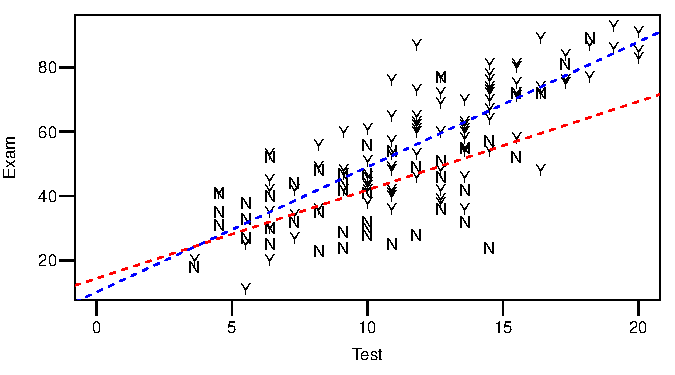
\includegraphics{figure/RC-H08-026}
\end{figure}

This a a visual confirmation of our intuition that the regular attenders get a `greater return' on their \rcode{Test} `investment'.

\end{frame}


\begin{frame}[fragile]
\frametitle{Fitting the interaction model directly with \rcode{lm}}
All that hard work we did with constructing \rcode{D} and \rcode{TestD} can be avoided
since \rcode{lm} will automatically do this for us.\\
\bigskip
We were interested to see whether the effect of \rcode{Test} interacts with the students \rcode{Attend} variable.
Using \rcode{lm} we simply specify \rcode{Test * Attend} to fit the model with interaction. That is,\\
\bigskip
%<<RC-H08-030, results = 'hide'>>=
\begin{knitrout}\scriptsize
\definecolor{shadecolor}{rgb}{0.969, 0.969, 0.969}\color{fgcolor}\begin{kframe}
\begin{alltt}
\hlstd{> }\hlstd{TestAttend.fit2}\hlkwb{=}\hlkwd{lm}\hlstd{(Exam}\hlopt{~}\hlstd{Test}\hlopt{*}\hlstd{Attend,} \hlkwc{data}\hlstd{=Stats20x.df)}
\hlstd{> }\hlkwd{summary}\hlstd{(TestAttend.fit2)}
\end{alltt}
\end{kframe}
\end{knitrout}
\begin{knitrout}\scriptsize
\definecolor{shadecolor}{rgb}{0.969, 0.969, 0.969}\color{fgcolor}\begin{kframe}
\begin{verbatim}
Coefficients:
               Estimate Std. Error t value Pr(>|t|)    
(Intercept)     14.4467     4.9443   2.922  0.00405 ** 
Test             2.7496     0.4603   5.973 1.78e-08 ***
AttendYes       -4.2582     6.3723  -0.668  0.50506    
Test:AttendYes   1.1380     0.5577   2.040  0.04316 *  
---
Residual standard error: 11.41 on 142 degrees of freedom
Multiple R-squared:  0.6347,	Adjusted R-squared:  0.627 
F-statistic: 82.25 on 3 and 142 DF,  p-value: < 2.2e-16
\end{verbatim}
\end{kframe}
\end{knitrout}
\end{frame}

%Must be factor
%Stats20x.df$Attend=relevel(Stats20x.df$Attend,ref="Yes")

\begin{frame}[fragile]
\frametitle{Fitting the interaction model directly with \rcode{lm}\dots}
Compare this with
\begin{knitrout}\scriptsize
\definecolor{shadecolor}{rgb}{0.969, 0.969, 0.969}\color{fgcolor}\begin{kframe}
\begin{alltt}
\hlstd{> }\hlkwd{Summary}\hlstd{(TestAttend.fit)}
\end{alltt}
\end{kframe}
\end{knitrout}
\begin{knitrout}\scriptsize
\definecolor{shadecolor}{rgb}{0.969, 0.969, 0.969}\color{fgcolor}\begin{kframe}
\begin{verbatim}
Coefficients:
            Estimate Std. Error t value Pr(>|t|)    
(Intercept)  14.4467     4.9443   2.922  0.00405 ** 
Test          2.7496     0.4603   5.973 1.78e-08 ***
D            -4.2582     6.3723  -0.668  0.50506    
TestD         1.1380     0.5577   2.040  0.04316 *  
---
Residual standard error: 11.41 on 142 degrees of freedom
Multiple R-squared:  0.6347,	Adjusted R-squared:  0.627 
F-statistic: 82.25 on 3 and 142 DF,  p-value: < 2.2e-16
\end{verbatim}
\end{kframe}
\end{knitrout}
\medskip
We have the same outputs, but with slightly different names.\\
\medskip
\textbf{Note:} \rcode{Test * Attend} is shorthand notation. You can be more explicit about the individual terms in the model by writing \\
\medskip
\begin{knitrout}\scriptsize
\definecolor{shadecolor}{rgb}{0.969, 0.969, 0.969}\color{fgcolor}\begin{kframe}
\begin{alltt}
\hlstd{> }\hlstd{TestAttend.fit2}\hlkwb{=}\hlkwd{lm}\hlstd{(Exam} \hlopt{~}\hlstd{Test} \hlopt{+} \hlstd{Attend} \hlopt{+} \hlstd{Test}\hlopt{:}\hlstd{Attend,} \hlkwc{data}\hlstd{=Stats20x.df)}
\end{alltt}
\end{kframe}
\end{knitrout}
We read this as, \emph{the effect of \rcode{Test}, plus the effect of \rcode{Attend}, plus the interaction between \rcode{Test} and \rcode{Attend}, which is denoted by \rcode{Test:Attend}}.

\end{frame}



%%%%%%%%%%%%%%%%%%%%%%%%%%%%%%%%%%%%%%%%%%%%%%%%%%%%%%%%%%%%%%%%%%%%%%%%%%%%%%%%%%%%%%%%%%%
\BeginSection{Interpretting the fitted model}
%%%%%%%%%%%%%%%%%%%%%%%%%%%%%%%%%%%%%%%%%%%%%%%%%%%%%%%%%%%%%%%%%%%%%%%%%%%%%%%%%%%%%%%%%%%


\begin{frame}[fragile]
\frametitle{Exam vs.\ test \textbf{and} attendance\ldots}
\framesubtitle{Let us take stock of this model}

\begin{knitrout}\scriptsize
\definecolor{shadecolor}{rgb}{0.969, 0.969, 0.969}\color{fgcolor}\begin{kframe}
\begin{alltt}
\hlstd{> }\hlkwd{summary}\hlstd{(TestAttend.fit2)}
\end{alltt}
\end{kframe}
\end{knitrout}
\begin{knitrout}\scriptsize
\definecolor{shadecolor}{rgb}{0.969, 0.969, 0.969}\color{fgcolor}\begin{kframe}
\begin{verbatim}
Coefficients:
               Estimate Std. Error t value Pr(>|t|)    
(Intercept)     14.4467     4.9443   2.922  0.00405 ** 
Test             2.7496     0.4603   5.973 1.78e-08 ***
AttendYes       -4.2582     6.3723  -0.668  0.50506    
Test:AttendYes   1.1380     0.5577   2.040  0.04316 *  
---
Residual standard error: 11.41 on 142 degrees of freedom
Multiple R-squared:  0.6347,	Adjusted R-squared:  0.627 
F-statistic: 82.25 on 3 and 142 DF,  p-value: < 2.2e-16
\end{verbatim}
\end{kframe}
\end{knitrout}
%typos bolded.
When we looked at the models that used explanatory variables \rcode{Test} and \rcode{Attend}
by themselves (in Chapter 2 \& 5 resp. ), they explained 59\% and 15\% of the variability of \rcode{Exam} respectively. 
When we use them together, we explain about \textbf{63}\% of the variability. 
\textbf{Why is it not $59+15 =74\%$?}. 

\medskip

It is because the addition of \rcode{Attend} can only explain variability that
has not already been explained by \rcode{Test}.
If \rcode{Attend} and \rcode{Test} are closely related then this may not be much --
this is called \textbf{multi-collinearity}.

\end{frame}


\begin{frame}[fragile]
\frametitle{Exam vs.\ test \textbf{and} attendance\ldots}
\framesubtitle{Let us take stock of this model\ldots}

We see that our intuition was correct. 
That is, the slope for \rcode{Test} of attenders is greater that for non-attenders. 
This is because the estimate of the difference in these slopes \rcode{TestD}.

\begin{knitrout}\scriptsize
\definecolor{shadecolor}{rgb}{0.969, 0.969, 0.969}\color{fgcolor}\begin{kframe}
\begin{alltt}
\hlstd{> }\hlkwd{coef}\hlstd{(TestAttend.fit2)[}\hlnum{4}\hlstd{]}
\end{alltt}
\begin{verbatim}
Test:AttendYes 
       1.13799 
\end{verbatim}
\end{kframe}
\end{knitrout}
is positive and statistically significant (\pval{} $\approx$ 0.04).\\
\bigskip
We were not sure about the differences in intercept and we see that this estimate is not significantly different from the hypothesised value of 0 (\pval{} $\approx$ 0.51).\\
\bigskip
Recall that we are not particularly interested in the null hypothesis $H_0: \beta_2=0$ when the slopes are different, so it is standard practice to leave this term in the model when $\beta_3$ is statistically significant.
\end{frame}


\begin{frame}[fragile]
\frametitle{Exam vs.\ test \textbf{and} attendance\ldots}
\framesubtitle{Let us take stock of this model\ldots}

The baseline slope that measures the effect of \rcode{Test} for non-attenders is statistically significant. 

\bigskip
The slope for attenders is significantly higher,
so we say that the effect of \rcode{Test} interacts with the \rcode{Attend} variable,
as the effect depends on the level of \rcode{Attend}.
\end{frame}




\begin{frame}[fragile]
\frametitle{Exam vs.\ test \textbf{and} attendance\ldots}
\framesubtitle{Some Inference}

Confidence intervals may be needed for the coefficients:\\
\bigskip
\begin{knitrout}\scriptsize
\definecolor{shadecolor}{rgb}{0.969, 0.969, 0.969}\color{fgcolor}\begin{kframe}
\begin{alltt}
\hlstd{> }\hlkwd{confint}\hlstd{(TestAttend.fit2)}
\end{alltt}
\begin{verbatim}
                      2.5 %    97.5 %
(Intercept)      4.67287511 24.220625
Test             1.83956971  3.659567
AttendYes      -16.85506294  8.338572
Test:AttendYes   0.03547053  2.240510
\end{verbatim}
\end{kframe}
\end{knitrout}
\bigskip \bigskip

\textbf{Recall:} Statistical significance (at the 5\% level) of a coefficient is equivalent to the (95\%) confidence interval \textbf{NOT} containing zero. 
\end{frame}


\begin{frame}[fragile]
\frametitle{Exam vs.\ test \textbf{and} attendance\ldots}
\framesubtitle{Some predictions}
\begin{knitrout}\scriptsize
\definecolor{shadecolor}{rgb}{0.969, 0.969, 0.969}\color{fgcolor}\begin{kframe}
\begin{alltt}
\hlstd{> }\hlstd{predTestAttend.df} \hlkwb{=} \hlkwd{data.frame}\hlstd{(}\hlkwc{Test} \hlstd{=} \hlkwd{c}\hlstd{(}\hlnum{0}\hlstd{,} \hlnum{10}\hlstd{,} \hlnum{10}\hlstd{,} \hlnum{20}\hlstd{),}
\hlstd{+ }                               \hlkwc{Attend} \hlstd{=} \hlkwd{factor}\hlstd{(}\hlkwd{c}\hlstd{(}\hlstr{"No"}\hlstd{,} \hlstr{"No"}\hlstd{,} \hlstr{"Yes"}\hlstd{,} \hlstr{"Yes"}\hlstd{))}
\hlstd{+ }                               \hlstd{)}
\hlstd{> }\hlstd{predTestAttend.df}
\end{alltt}
\begin{verbatim}
  Test Attend
1    0     No
2   10     No
3   10    Yes
4   20    Yes
\end{verbatim}
\end{kframe}
\end{knitrout}
\bigskip
Let us estimate the expected exam scores for these values of test score and attendance:\\
\bigskip
\begin{knitrout}\scriptsize
\definecolor{shadecolor}{rgb}{0.969, 0.969, 0.969}\color{fgcolor}\begin{kframe}
\begin{alltt}
\hlstd{> }\hlkwd{predict}\hlstd{(TestAttend.fit2,predTestAttend.df,} \hlkwc{interval}\hlstd{=}\hlstr{"confidence"}\hlstd{)}
\end{alltt}
\begin{verbatim}
       fit       lwr      upr
1 14.44675  4.672875 24.22062
2 41.94243 38.616376 45.26849
3 49.06409 46.412194 51.71599
4 87.93968 82.610100 93.26926
\end{verbatim}
\end{kframe}
\end{knitrout}
\end{frame}


\begin{frame}[fragile]
\frametitle{Exam vs.\ test \textbf{and} attendance\ldots}
\framesubtitle{Some predictions\ldots}
Now, let us predict the exam score for individual students with those test scores
and attendance:\\
\medskip
\begin{knitrout}\scriptsize
\definecolor{shadecolor}{rgb}{0.969, 0.969, 0.969}\color{fgcolor}\begin{kframe}
\begin{alltt}
\hlstd{> }\hlkwd{predict}\hlstd{(TestAttend.fit2,predTestAttend.df,} \hlkwc{interval}\hlstd{=}\hlstr{"prediction"}\hlstd{)}
\end{alltt}
\begin{verbatim}
       fit       lwr       upr
1 14.44675 -10.13028  39.02378
2 41.94243  19.14848  64.73639
3 49.06409  26.35871  71.76947
4 87.93968  64.76845 111.11092
\end{verbatim}
\end{kframe}
\end{knitrout}
\medskip
This is not the best model for predicting individual student exam scores as the intervals are too wide and in some case are meaningless (at the extremes of \rcode{Test}). \\
\medskip
This is related to the fact that we can only explain 63\% of the variability in \rcode{Exam} or, equivalently, we can not account for 37\% of this variability. Also, our linear model does not ``know'' about the constraint that exam scores must be between 0 and 100.
\end{frame}


\begin{frame}[fragile]
\frametitle{Exam vs.\ test \textbf{and} attendance\ldots}
\framesubtitle{Methods and assumption checks}

A plot of the data showed that exam scores appear to increase linearly with test score,
but with different lines for attenders and non-attenders.\\
\bigskip
The model with interaction was fitted and the attendance/test score interaction was found to be significant.\footnote{See the Case Study for the model equation.}\\
\bigskip
The students should be acting independently of each other as this was an exam.\\
\bigskip
The EOV assumption appears to be reasonable notwithstanding some reduced variability at the high end of test and exam scores.
The data also look approximately normal.
There do not appear to be any unduly influential data points. \\
\bigskip 
Our model explains 63\% of the total variability in exam scores.
\end{frame}


\begin{frame}[fragile]
\frametitle{Exam vs.\ test \textbf{and} attendance\ldots}
\framesubtitle{Executive summary}
There is a clear linear relationship between Test and Exam, but it differs in strength between  non-attenders and attenders.\\
\bigskip
We estimate that each additional test mark (out of 20) will increase the expected exam mark
  of a non-attender by 1.8 to 3.7.\\
  \bigskip
There is a further increase of between 0 to 2.2 marks for regular attenders.\\
\bigskip
\textbf{Note:} In an assignment or exam situation you might also be required to comment on additional confidence and/or prediction intervals---this will be made clear in the instructions.
\end{frame}



\begin{frame}[fragile]
\frametitle{Exam vs.\ test \textbf{and} attendance\ldots}
\framesubtitle{Executive summary...}
Note that the above Executive Summary is missing the confidence interval for the effect of test mark on attenders. To obtain this CI we need to change attenders to the baseline level of \rcode{Attend}.
\medskip
\begin{knitrout}\scriptsize
\definecolor{shadecolor}{rgb}{0.969, 0.969, 0.969}\color{fgcolor}\begin{kframe}
\begin{alltt}
\hlstd{> }\hlstd{Stats20x.df}\hlopt{$}\hlstd{Attend2}\hlkwb{=}\hlkwd{relevel}\hlstd{(Stats20x.df}\hlopt{$}\hlstd{Attend,}\hlkwc{ref}\hlstd{=}\hlstr{"Yes"}\hlstd{)}
\hlstd{> }\hlstd{TestAttend.fit2b}\hlkwb{=}\hlkwd{lm}\hlstd{(Exam} \hlopt{~}\hlstd{Test}\hlopt{*}\hlstd{Attend2,} \hlkwc{data}\hlstd{=Stats20x.df)}
\hlstd{> }\hlkwd{coef}\hlstd{(}\hlkwd{summary}\hlstd{(TestAttend.fit2b))}
\end{alltt}
\begin{verbatim}
                Estimate Std. Error    t value     Pr(>|t|)
(Intercept)    10.188504  4.0199956  2.5344566 1.234648e-02
Test            3.887559  0.3148792 12.3461898 3.020895e-24
Attend2No       4.258246  6.3722922  0.6682439 5.050626e-01
Test:Attend2No -1.137990  0.5577265 -2.0404094 4.316270e-02
\end{verbatim}
\begin{alltt}
\hlstd{> }\hlkwd{confint}\hlstd{(TestAttend.fit2b)}
\end{alltt}
\begin{verbatim}
                   2.5 %      97.5 %
(Intercept)     2.241733 18.13527583
Test            3.265102  4.51001561
Attend2No      -8.338572 16.85506294
Test:Attend2No -2.240510 -0.03547053
\end{verbatim}
\end{kframe}
\end{knitrout}

We estimate that each additional test mark will increase the expected exam mark
of an attender by 3.3 to 4.5.\\
\end{frame}


%%%%%%%%%%%%%%%%%%%%%%%%%%%%%%%%%%%%%%%%%%%%%%%%%%%%%%%%%%%%%%%%%%%%%%%%%%%%%%%%%%%%%%%%%%%
\BeginSection{Assessing influence of the atypical students}
%%%%%%%%%%%%%%%%%%%%%%%%%%%%%%%%%%%%%%%%%%%%%%%%%%%%%%%%%%%%%%%%%%%%%%%%%%%%%%%%%%%%%%%%%%%


\begin{frame}[fragile]
\frametitle{Exam vs.\ test \textbf{and} attendance\ldots}
\framesubtitle{Sensitivity check}

In the exploratory phase of the analysis we identified three students as being potentially anomolous. Recall, these were the 3 non-attending students who scored greater than 16 on the test.\\
\bigskip
If we have reason to think these students are `atypical' (do we?) then it might make sense to do the analysis without them.\\ 
\bigskip
What do you think happens to our respective straight lines?\\
\bigskip
Let us see what happens. We will pull these three students out of the dataframe. 
\medskip
\begin{knitrout}\scriptsize
\definecolor{shadecolor}{rgb}{0.969, 0.969, 0.969}\color{fgcolor}\begin{kframe}
\begin{alltt}
\hlstd{> }\hlcom{## Remove atypical points - Note that ! means 'not'}
\hlstd{> }\hlstd{Subset.df}\hlkwb{=}\hlkwd{subset}\hlstd{(Stats20x.df,} \hlopt{!}\hlstd{(Test}\hlopt{>}\hlnum{16}\hlopt{&}\hlstd{Attend}\hlopt{==}\hlstr{"No"}\hlstd{))}
\hlstd{> }\hlstd{TestAttend.fit3}\hlkwb{=}\hlkwd{lm}\hlstd{(Exam} \hlopt{~}\hlstd{Test}\hlopt{*}\hlstd{Attend,} \hlkwc{data}\hlstd{=Subset.df)}
\hlstd{> }\hlkwd{summary}\hlstd{(TestAttend.fit3)}
\end{alltt}
\end{kframe}
\end{knitrout}
\end{frame}


\begin{frame}[fragile]
\frametitle{Exam vs.\ test \textbf{and} attendance\ldots}
\framesubtitle{Sensitivity check\ldots}
\begin{knitrout}\scriptsize
\definecolor{shadecolor}{rgb}{0.969, 0.969, 0.969}\color{fgcolor}\begin{kframe}
\begin{verbatim}
Coefficients:
               Estimate Std. Error t value Pr(>|t|)    
(Intercept)     22.6522     5.2776   4.292  3.3e-05 ***
Test             1.7590     0.5213   3.374 0.000960 ***
AttendYes      -12.4637     6.5505  -1.903 0.059146 .  
Test:AttendYes   2.1285     0.6034   3.527 0.000569 ***
---
Residual standard error: 11.01 on 139 degrees of freedom
Multiple R-squared:  0.6495,	Adjusted R-squared:  0.6419 
F-statistic: 85.86 on 3 and 139 DF,  p-value: < 2.2e-16
\end{verbatim}
\end{kframe}
\end{knitrout}
\bigskip
Note that we have smaller degrees of freedom as we have 3 fewer data points. 
Look at how the parameters have changed.
\medskip

Our $R^2$ value has increased slightly as we have less variability overall.
\end{frame}


\begin{frame}[fragile]
\frametitle{Exam vs.\ test \textbf{and} attendance\ldots}
\framesubtitle{Sensitivity check\ldots}

\rcode{R} code to generate the plot of the full data with all three of the fitted lines:
\begin{knitrout}\scriptsize
\definecolor{shadecolor}{rgb}{0.969, 0.969, 0.969}\color{fgcolor}\begin{kframe}
\begin{alltt}
\hlstd{> }\hlcom{## Plot these data all together}
\hlstd{> }\hlkwd{plot}\hlstd{(Exam} \hlopt{~} \hlstd{Test,} \hlkwc{data} \hlstd{= Subset.df,}\hlkwc{pch} \hlstd{=} \hlkwd{substr}\hlstd{(Attend,} \hlnum{1}\hlstd{,} \hlnum{1}\hlstd{),}\hlkwc{cex} \hlstd{=} \hlnum{0.7}\hlstd{)}
\hlstd{> }
\hlstd{> }\hlcom{## Remember that we've defined b in Slide 26}
\hlstd{> }\hlcom{## Each abline() will have a different colour}
\hlstd{> }\hlkwd{abline}\hlstd{(b[}\hlnum{1}\hlopt{:}\hlnum{2}\hlstd{],} \hlkwc{lty} \hlstd{=} \hlnum{2}\hlstd{,} \hlkwc{col} \hlstd{=} \hlstr{"red"}\hlstd{)}
\hlstd{> }\hlkwd{abline}\hlstd{(b[}\hlnum{1}\hlstd{]} \hlopt{+} \hlstd{b[}\hlnum{3}\hlstd{], b[}\hlnum{2}\hlstd{]} \hlopt{+} \hlstd{b[}\hlnum{4}\hlstd{],} \hlkwc{lty} \hlstd{=} \hlnum{2}\hlstd{,} \hlkwc{col} \hlstd{=} \hlstr{"blue"}\hlstd{)}
\hlstd{> }
\hlstd{> }\hlcom{## The fitted line without the 3 atypical points}
\hlstd{> }\hlstd{b2} \hlkwb{=} \hlkwd{coef}\hlstd{(TestAttend.fit3)} \hlcom{## Easier to work with these terms}
\hlstd{> }\hlkwd{abline}\hlstd{(b2[}\hlnum{1}\hlopt{:}\hlnum{2}\hlstd{],} \hlkwc{lty} \hlstd{=} \hlnum{2}\hlstd{,} \hlkwc{col} \hlstd{=} \hlstr{"green"}\hlstd{)}
\hlstd{> }
\hlstd{> }\hlcom{## Add a legend to help us differentiate between the lines for non-attenders}
\hlstd{> }\hlkwd{legend}\hlstd{(}\hlstr{"topleft"}\hlstd{,} \hlkwc{legend} \hlstd{=} \hlkwd{c}\hlstd{(}\hlstr{"All non-attenders"}\hlstd{,} \hlstr{"Without atypical non-attenders"}\hlstd{),}
\hlstd{+ }       \hlkwc{lty} \hlstd{=} \hlnum{2}\hlstd{,} \hlkwc{col} \hlstd{=} \hlkwd{c}\hlstd{(}\hlstr{"red"}\hlstd{,} \hlstr{"green"}\hlstd{),} \hlkwc{bty} \hlstd{=} \hlstr{"n"}\hlstd{)}
\end{alltt}
\end{kframe}
\end{knitrout}

\end{frame}


\begin{frame}[fragile, t]
\frametitle{Exam vs.\ test \textbf{and} attendance\ldots} 
\framesubtitle{Sensitivity check\ldots}


% c(, , , )

\begin{figure}
  \centering
  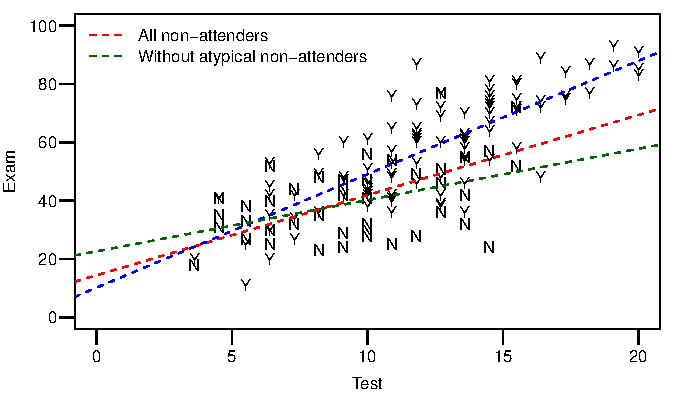
\includegraphics{figure/RC-H08-040}
\end{figure}

Comments?
\end{frame}



%%%%%%%%%%%%%%%%%%%%%%%%%%%%%%%%%%%%%%%%%%%%%%%%%%%%%%%%%%%%%%%%%%%%%%%%%%%%%%%%%%%%%%%%%%%
\BeginSection{Some insight and relevant \rcode{R}-code.}
%%%%%%%%%%%%%%%%%%%%%%%%%%%%%%%%%%%%%%%%%%%%%%%%%%%%%%%%%%%%%%%%%%%%%%%%%%%%%%%%%%%%%%%%%%%



\begin{frame}[fragile]
\frametitle{\rcode{R} tips and tricks}
\framesubtitle{\rcode{model.matrix}}

Recall that \rcode{lm} automatically created the necessary indicator variables to fit the above 
models.

\medskip

To explicitly see the model formula that \rcode{lm} is using, we only have to ask:

\begin{knitrout}\scriptsize
\definecolor{shadecolor}{rgb}{0.969, 0.969, 0.969}\color{fgcolor}\begin{kframe}
\begin{alltt}
\hlstd{> }\hlstd{ModMat}\hlkwb{=}\hlkwd{model.matrix}\hlstd{(}\hlopt{~}\hlstd{Test}\hlopt{*}\hlstd{Attend,}\hlkwc{data}\hlstd{=Stats20x.df)}
\hlstd{> }\hlkwd{cbind}\hlstd{(Stats20x.df[,}\hlkwd{c}\hlstd{(}\hlstr{"Test"}\hlstd{,}\hlstr{"Attend"}\hlstd{)],ModMat)[}\hlnum{1}\hlopt{:}\hlnum{10}\hlstd{,]}
\end{alltt}
\begin{verbatim}
   Test Attend (Intercept) Test AttendYes Test:AttendYes
1   9.1    Yes           1  9.1         1            9.1
2  13.6    Yes           1 13.6         1           13.6
3  14.5    Yes           1 14.5         1           14.5
4  19.1    Yes           1 19.1         1           19.1
5   8.2     No           1  8.2         0            0.0
6  12.7    Yes           1 12.7         1           12.7
7   7.3    Yes           1  7.3         1            7.3
8  10.9     No           1 10.9         0            0.0
9  10.9    Yes           1 10.9         1           10.9
10  9.1    Yes           1  9.1         1            9.1
\end{verbatim}
\end{kframe}
\end{knitrout}

\medskip
The \rcode{AttendYes} variable is \rcode{D},
and \rcode{Test:AttendYes} is $\rcode{D} \times \rcode{Test}$.
\end{frame}



\begin{frame}[fragile]
\frametitle{Most of the \rcode{R}-code you need for this chapter}

As always, your code requires the usual code (data exploration, etc) and model checks discussed in chapters 1 and 2.\footnote{That is, until we reach Chapter 13.}

\medskip
When $y$ can be explained by a categorical (i.e., factor) variable and also a numeric (i.e., continuous) variable then you can use both.
\medskip

You do not need to create indicator variables as \rcode{R} does this for you. It will choose the baseline for you, so be careful.  You can change this if needed, using the \rcode{relevel} function. 
\medskip


Fit as follows:

\begin{knitrout}\scriptsize
\definecolor{shadecolor}{rgb}{0.969, 0.969, 0.969}\color{fgcolor}\begin{kframe}
\begin{alltt}
\hlstd{> }\hlstd{TestAttend.fit2}\hlkwb{=}\hlkwd{lm}\hlstd{(Exam} \hlopt{~}\hlstd{Test}\hlopt{*}\hlstd{Attend,} \hlkwc{data}\hlstd{=Stats20x.df)}
\hlstd{> }\hlcom{#check to see it's okay}
\hlstd{> }\hlkwd{plot}\hlstd{(TestAttend.fit2,} \hlkwc{which}\hlstd{=}\hlnum{1}\hlstd{)} \hlcom{#followed by normcheck and cooks20x}
\hlstd{> }\hlcom{# then see if you need a separate slope for each level of your factor var.}
\hlstd{> }\hlkwd{summary}\hlstd{(TestAttend.fit2)}
\end{alltt}
\end{kframe}
\end{knitrout}

Interpret accordingly. In particular, if the interaction term is not significant then proceed to the next Chapter.

\end{frame}



\end{document}

